\documentclass{standalone}
\usepackage{tikz}
\usetikzlibrary{patterns, positioning}


\begin{document}
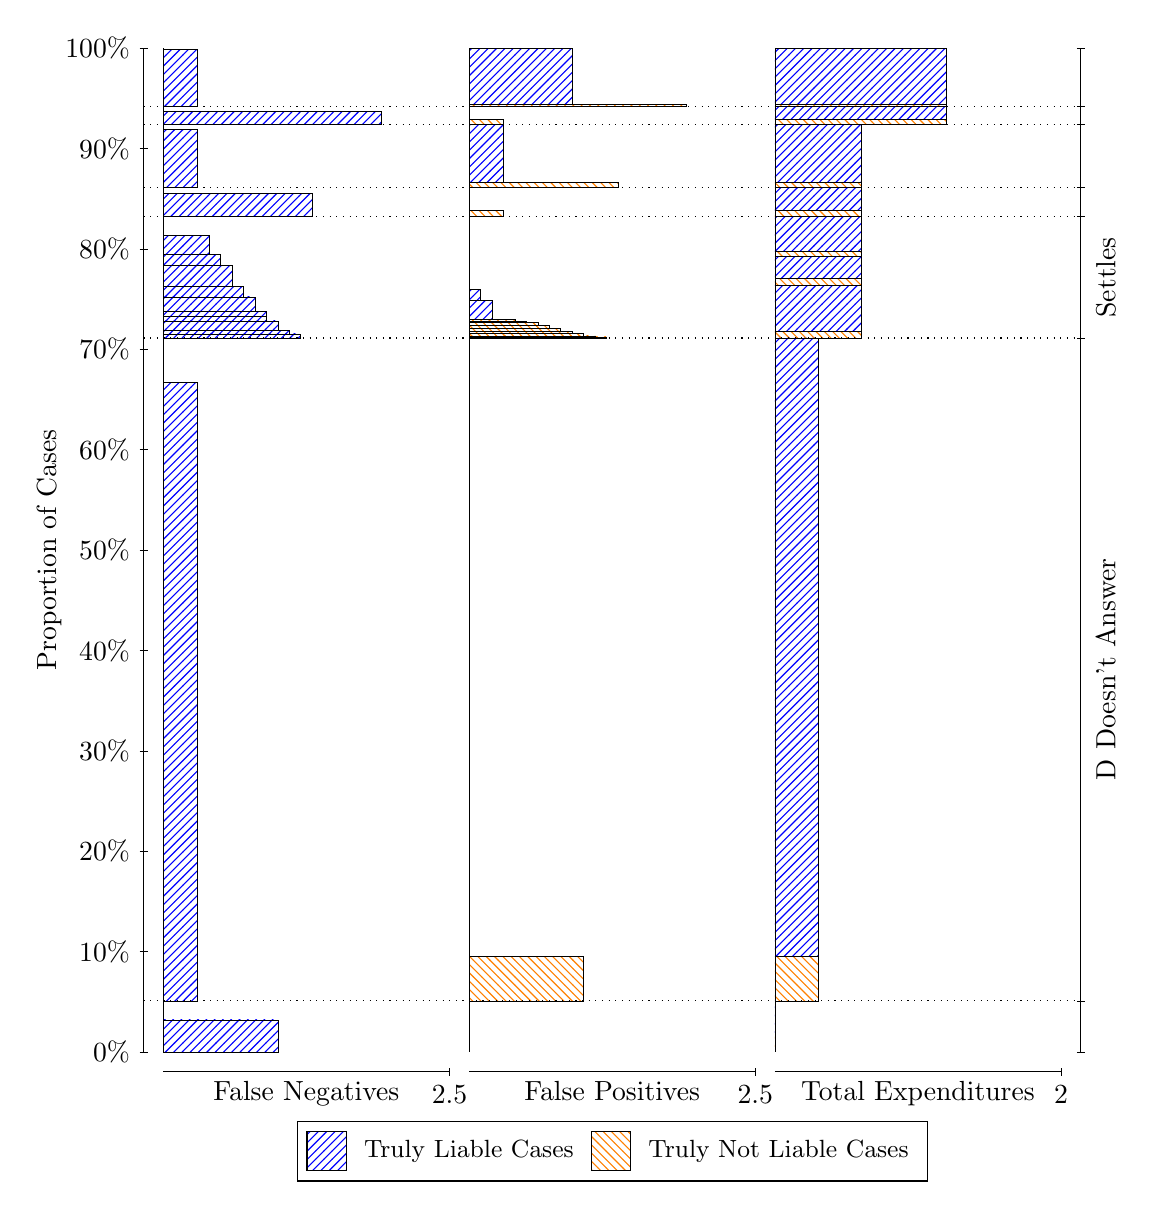
\begin{tikzpicture}
\draw[black, very thin] (1.5,1.75) -- (1.5,14.5);
\node[rotate=90, text=black, anchor=center] at (0.3, 8.125) {Proportion of Cases};
\draw[black, very thin] (1.45,1.75) -- (1.55,1.75);
\node[text=black, anchor=east] at (1.45, 1.75) {0\%};
\draw[black, very thin] (1.45,3.025) -- (1.55,3.025);
\node[text=black, anchor=east] at (1.45, 3.025) {10\%};
\draw[black, very thin] (1.45,4.3) -- (1.55,4.3);
\node[text=black, anchor=east] at (1.45, 4.3) {20\%};
\draw[black, very thin] (1.45,5.575) -- (1.55,5.575);
\node[text=black, anchor=east] at (1.45, 5.575) {30\%};
\draw[black, very thin] (1.45,6.85) -- (1.55,6.85);
\node[text=black, anchor=east] at (1.45, 6.85) {40\%};
\draw[black, very thin] (1.45,8.125) -- (1.55,8.125);
\node[text=black, anchor=east] at (1.45, 8.125) {50\%};
\draw[black, very thin] (1.45,9.4) -- (1.55,9.4);
\node[text=black, anchor=east] at (1.45, 9.4) {60\%};
\draw[black, very thin] (1.45,10.675) -- (1.55,10.675);
\node[text=black, anchor=east] at (1.45, 10.675) {70\%};
\draw[black, very thin] (1.45,11.95) -- (1.55,11.95);
\node[text=black, anchor=east] at (1.45, 11.95) {80\%};
\draw[black, very thin] (1.45,13.225) -- (1.55,13.225);
\node[text=black, anchor=east] at (1.45, 13.225) {90\%};
\draw[black, very thin] (1.45,14.5) -- (1.55,14.5);
\node[text=black, anchor=east] at (1.45, 14.5) {100\%};

\draw[black, very thin] (13.4,1.75) -- (13.4,14.5);
\draw[black, very thin] (13.35,1.75) -- (13.45,1.75);
\node[anchor=west] at (13.35, 1.75) {};
\draw[black, very thin] (13.35,2.3989) -- (13.45,2.3989);
\node[anchor=west] at (13.35, 2.3989) {};
\draw[black, very thin] (13.35,10.818) -- (13.45,10.818);
\node[anchor=west] at (13.35, 10.818) {};
\draw[black, very thin] (13.35,12.359) -- (13.45,12.359);
\node[anchor=west] at (13.35, 12.359) {};
\draw[black, very thin] (13.35,12.733) -- (13.45,12.733);
\node[anchor=west] at (13.35, 12.733) {};
\draw[black, very thin] (13.35,13.527) -- (13.45,13.527);
\node[anchor=west] at (13.35, 13.527) {};
\draw[black, very thin] (13.35,13.761) -- (13.45,13.761);
\node[anchor=west] at (13.35, 13.761) {};
\draw[black, very thin] (13.35,14.5) -- (13.45,14.5);
\node[anchor=west] at (13.35, 14.5) {};

\draw[black, very thin, pattern color=blue, pattern=north east lines] (1.75,1.75) rectangle (3.2033,2.1577);
\draw[black, very thin, pattern color=orange, pattern=north west lines] (1.75,2.1577) rectangle (1.75,2.3989);
\draw[black, very thin, pattern color=blue, pattern=north east lines] (1.75,2.3989) rectangle (2.186,10.251);
\draw[black, very thin, pattern color=orange, pattern=north west lines] (1.75,10.251) rectangle (1.75,10.818);
\draw[black, very thin, pattern color=blue, pattern=north east lines] (1.75,10.818) rectangle (3.494,10.87);
\draw[black, very thin, pattern color=blue, pattern=north east lines] (1.75,10.87) rectangle (3.3487,10.918);
\draw[black, very thin, pattern color=blue, pattern=north east lines] (1.75,10.918) rectangle (3.2033,11.035);
\draw[black, very thin, pattern color=blue, pattern=north east lines] (1.75,11.035) rectangle (3.058,11.091);
\draw[black, very thin, pattern color=blue, pattern=north east lines] (1.75,11.091) rectangle (3.058,11.159);
\draw[black, very thin, pattern color=blue, pattern=north east lines] (1.75,11.159) rectangle (2.9127,11.339);
\draw[black, very thin, pattern color=blue, pattern=north east lines] (1.75,11.339) rectangle (2.7673,11.472);
\draw[black, very thin, pattern color=blue, pattern=north east lines] (1.75,11.472) rectangle (2.622,11.743);
\draw[black, very thin, pattern color=blue, pattern=north east lines] (1.75,11.743) rectangle (2.4767,11.878);
\draw[black, very thin, pattern color=blue, pattern=north east lines] (1.75,11.878) rectangle (2.3313,12.12);
\draw[black, very thin, pattern color=orange, pattern=north west lines] (1.75,12.12) rectangle (1.75,12.359);
\draw[black, very thin, pattern color=blue, pattern=north east lines] (1.75,12.359) rectangle (3.6393,12.651);
\draw[black, very thin, pattern color=orange, pattern=north west lines] (1.75,12.651) rectangle (1.75,12.733);
\draw[black, very thin, pattern color=blue, pattern=north east lines] (1.75,12.733) rectangle (2.186,13.466);
\draw[black, very thin, pattern color=orange, pattern=north west lines] (1.75,13.466) rectangle (1.75,13.527);
\draw[black, very thin, pattern color=blue, pattern=north east lines] (1.75,13.527) rectangle (4.5113,13.696);
\draw[black, very thin, pattern color=orange, pattern=north west lines] (1.75,13.696) rectangle (1.75,13.761);
\draw[black, very thin, pattern color=blue, pattern=north east lines] (1.75,13.761) rectangle (2.186,14.481);
\draw[black, very thin, pattern color=orange, pattern=north west lines] (1.75,14.481) rectangle (1.75,14.5);
\draw[black, very thin, pattern color=orange, pattern=north west lines] (5.6333,1.75) rectangle (5.6333,1.9912);
\draw[black, very thin, pattern color=blue, pattern=north east lines] (5.6333,1.9912) rectangle (5.6333,2.3989);
\draw[black, very thin, pattern color=orange, pattern=north west lines] (5.6333,2.3989) rectangle (7.0867,2.9661);
\draw[black, very thin, pattern color=blue, pattern=north east lines] (5.6333,2.9661) rectangle (5.6333,10.818);
\draw[black, very thin, pattern color=orange, pattern=north west lines] (5.6333,10.818) rectangle (7.3773,10.832);
\draw[black, very thin, pattern color=orange, pattern=north west lines] (5.6333,10.832) rectangle (7.232,10.845);
\draw[black, very thin, pattern color=orange, pattern=north west lines] (5.6333,10.845) rectangle (7.0867,10.872);
\draw[black, very thin, pattern color=orange, pattern=north west lines] (5.6333,10.872) rectangle (6.9413,10.901);
\draw[black, very thin, pattern color=orange, pattern=north west lines] (5.6333,10.901) rectangle (6.796,10.944);
\draw[black, very thin, pattern color=orange, pattern=north west lines] (5.6333,10.944) rectangle (6.6507,10.978);
\draw[black, very thin, pattern color=orange, pattern=north west lines] (5.6333,10.978) rectangle (6.5053,11.016);
\draw[black, very thin, pattern color=orange, pattern=north west lines] (5.6333,11.016) rectangle (6.36,11.032);
\draw[black, very thin, pattern color=orange, pattern=north west lines] (5.6333,11.032) rectangle (6.2147,11.057);
\draw[black, very thin, pattern color=blue, pattern=north east lines] (5.6333,11.057) rectangle (5.924,11.299);
\draw[black, very thin, pattern color=blue, pattern=north east lines] (5.6333,11.299) rectangle (5.7787,11.433);
\draw[black, very thin, pattern color=blue, pattern=north east lines] (5.6333,11.433) rectangle (5.6333,12.359);
\draw[black, very thin, pattern color=orange, pattern=north west lines] (5.6333,12.359) rectangle (6.0693,12.441);
\draw[black, very thin, pattern color=blue, pattern=north east lines] (5.6333,12.441) rectangle (5.6333,12.733);
\draw[black, very thin, pattern color=orange, pattern=north west lines] (5.6333,12.733) rectangle (7.5227,12.794);
\draw[black, very thin, pattern color=blue, pattern=north east lines] (5.6333,12.794) rectangle (6.0693,13.527);
\draw[black, very thin, pattern color=orange, pattern=north west lines] (5.6333,13.527) rectangle (6.0693,13.592);
\draw[black, very thin, pattern color=blue, pattern=north east lines] (5.6333,13.592) rectangle (5.6333,13.761);
\draw[black, very thin, pattern color=orange, pattern=north west lines] (5.6333,13.761) rectangle (8.3947,13.78);
\draw[black, very thin, pattern color=blue, pattern=north east lines] (5.6333,13.78) rectangle (6.9413,14.5);
\draw[black, very thin, pattern color=orange, pattern=north west lines] (9.5167,1.75) rectangle (9.5167,1.9912);
\draw[black, very thin, pattern color=blue, pattern=north east lines] (9.5167,1.9912) rectangle (9.5167,2.3989);
\draw[black, very thin, pattern color=orange, pattern=north west lines] (9.5167,2.3989) rectangle (10.062,2.9661);
\draw[black, very thin, pattern color=blue, pattern=north east lines] (9.5167,2.9661) rectangle (10.062,10.818);
\draw[black, very thin, pattern color=orange, pattern=north west lines] (9.5167,10.818) rectangle (10.607,10.901);
\draw[black, very thin, pattern color=blue, pattern=north east lines] (9.5167,10.901) rectangle (10.607,11.488);
\draw[black, very thin, pattern color=orange, pattern=north west lines] (9.5167,11.488) rectangle (10.607,11.578);
\draw[black, very thin, pattern color=blue, pattern=north east lines] (9.5167,11.578) rectangle (10.607,11.851);
\draw[black, very thin, pattern color=orange, pattern=north west lines] (9.5167,11.851) rectangle (10.607,11.916);
\draw[black, very thin, pattern color=blue, pattern=north east lines] (9.5167,11.916) rectangle (10.607,12.359);
\draw[black, very thin, pattern color=orange, pattern=north west lines] (9.5167,12.359) rectangle (10.607,12.441);
\draw[black, very thin, pattern color=blue, pattern=north east lines] (9.5167,12.441) rectangle (10.607,12.733);
\draw[black, very thin, pattern color=orange, pattern=north west lines] (9.5167,12.733) rectangle (10.607,12.794);
\draw[black, very thin, pattern color=blue, pattern=north east lines] (9.5167,12.794) rectangle (10.607,13.527);
\draw[black, very thin, pattern color=orange, pattern=north west lines] (9.5167,13.527) rectangle (11.697,13.592);
\draw[black, very thin, pattern color=blue, pattern=north east lines] (9.5167,13.592) rectangle (11.697,13.761);
\draw[black, very thin, pattern color=orange, pattern=north west lines] (9.5167,13.761) rectangle (11.697,13.78);
\draw[black, very thin, pattern color=blue, pattern=north east lines] (9.5167,13.78) rectangle (11.697,14.5);
\draw[black, dotted] (1.5,2.3989) -- (13.4,2.3989);
\draw[black, dotted] (1.5,10.818) -- (13.4,10.818);
\draw[black, dotted] (1.5,12.359) -- (13.4,12.359);
\draw[black, dotted] (1.5,12.733) -- (13.4,12.733);
\draw[black, dotted] (1.5,13.527) -- (13.4,13.527);
\draw[black, dotted] (1.5,13.761) -- (13.4,13.761);
\draw[black, very thin] (1.75,1.5) -- (5.3833,1.5);
\node[text=black, anchor=north] at (3.5667, 1.5) {False Negatives};
\draw[black, very thin] (5.3833,1.45) -- (5.3833,1.55);
\node[text=black, anchor=north] at (5.3833, 1.45) {2.5};

\draw[black, very thin] (5.6333,1.5) -- (9.2667,1.5);
\node[text=black, anchor=north] at (7.45, 1.5) {False Positives};
\draw[black, very thin] (9.2667,1.45) -- (9.2667,1.55);
\node[text=black, anchor=north] at (9.2667, 1.45) {2.5};

\draw[black, very thin] (9.5167,1.5) -- (13.15,1.5);
\node[text=black, anchor=north] at (11.333, 1.5) {Total Expenditures};
\draw[black, very thin] (13.15,1.45) -- (13.15,1.55);
\node[text=black, anchor=north] at (13.15, 1.45) {2};


\node[text=black, centered, rotate=90] at (13.72, 6.6086) {D Doesn't Answer};
\node[text=black, centered, rotate=90] at (13.72, 11.588) {Settles};





\draw (7.449999999999999,1.5) node[draw=none] (baseCoordinate) {};
\begin{scope}[align=center]
        \matrix[scale=0.5, draw=black, below=0.5cm of baseCoordinate, nodes={draw}, column sep=0.1cm]{
            \node[rectangle, draw, minimum width=0.5cm, minimum height=0.5cm, pattern color=blue, pattern=north east lines] {}; &
            \node[draw=none, font=\small, text=black] (B) {Truly Liable Cases}; &
            \node[rectangle, draw, minimum width=0.5cm, minimum height=0.5cm, pattern color=orange, pattern=north west lines] {}; &
            \node[draw=none, font=\small, text=black] (B) {Truly Not Liable Cases}; \\
            };
\end{scope}

\end{tikzpicture}
\end{document}